\documentclass{bioinfo}
\copyrightyear{2017} \pubyear{2017}
\usepackage[english]{babel}
\usepackage{float}
\usepackage{graphicx}
\usepackage{amsmath}
\usepackage{multirow}
\usepackage{color}

\access{Advance Access Publication Date: Day Month Year}
\appnotes{Original Paper}

\begin{document}
\firstpage{1}

\subtitle{Structural bioinformatics}

\title[short Title]{Deep convolutional networks for quality assessment of protein folds}
\author[G. Derevyanko \textit{et~al}.]{Georgy Derevyanko\,$^{\text{\sfb 1,}*}$, Sergei Grudinin\,$^{\text{\sfb 2}}$, Yoshua Bengio\,$^{\text{\sfb 3}}$ and Guillaume Lamoureux\,$^{\text{\sfb 1,}*}$}
\address{$^{\text{\sf 1}}$Department of Chemistry and Biochemistry and Centre for Research in Molecular Modeling (CERMM), Concordia University, Montr{\'e}al, H4B 1R6, Canada,
$^{\text{\sf 2}}$Department, Institution, City, Post Code, France and
$^{\text{\sf 3}}$Department of Computer Science and Operations Research, Universit{\'e} de Montr{\'e}al, Montr{\'e}al, H3C 3J7, Canada.}

\corresp{$^\ast$To whom correspondence should be addressed.}

\history{Received on XXXXX; revised on XXXXX; accepted on XXXXX}

\editor{Associate Editor: XXXXXXX}

\abstract{\textbf{Motivation:} The computational prediction of a protein structure from its sequence
generally relies on a method to assess the quality of protein
models. However, most state-of-the-art assessment methods rank
candidate models using heavily engineered structural features. This work also suggests that it is
possible to include to the assessment algorithm other important
three-dimensional information such as electrostatic potential or
solute distribution.\\
\textbf{Results:} In this
work, we show that deep convolutional networks can be used to predict
the ranking of model structures solely on the basis of their raw
three-dimensional atomic densities, without any feature tuning. We
develop a deep neural network that performs on par with the best
algorithms from the literature.\\
\textbf{Availability:} The code as well and the preprocessed datasets available at \href{proteinfoldingproject.com}{proteinfoldingproject.com}.\\
\textbf{Contact:} \href{georgy.derevyanko@gmail.com}{georgy.derevyanko@gmail.com or \href{guillaume.lamoureux@concordia.ca}{guillaume.lamoureux@concordia.ca}}\\
\textbf{Supplementary information:} Supplementary data are available at \textit{Bioinformatics}
online.}

\maketitle

\section{Introduction}

The protein folding problem remains one of the outstanding challenges
in structural biology \citep{dill2012folding}.  It is usually defined
as the task of predicting the three-dimensional (3D) structure of a
protein from its amino acid sequence. A crucial step when making such
prediction is the ranking of candidate structures. Given a number of
structural models, can we computationally predict how close each of
them is to the unknown native fold of the protein?

Progress in the field is monitored through the Critical Assessment of
protein Structure Prediction (CASP) competition \citep{moult1995large},
in which protein folding methods are evaluated in terms of their
accuracy at predicting protein structures ahead of their
publication. Most methods in competition include a conformational
sampling step, which generates a number of plausible protein
conformations, and a quality assessment step, which attempts to select
the conformations closest to the unknown native structure.

In this work we explore the application of deep learning to the
problem of ``model quality assessment'' (MQA), also called
``estimation of model accuracy'' (EMA) \citep{kryshtafovych2015}. Deep
learning (DL) has recently garnered considerable interest in the
research community \citep{lecun2015deep}, particularly in computer
vision and natural language processing. Unlike more ``shallow''
machine learning approaches, deep learning improves performance by
learning a hierarchical representation of the raw data at hand. It
alleviates the need for feature engineering, which has traditionally
constituted the bulk of the work done by researchers.

Deep learning has recently been applied to biological data and has
yielded remarkable results for predicting the effects of genetic
variations on human RNA splicing \citep{xiong2015human}, for
identifying DNA- and RNA-binding
motifs \citep{alipanahi2015predicting}, and for predicting the effects
of non-coding DNA variants with single nucleotide
precision \citep{zhou2015predicting}. These successes have one thing in
common: they use raw data directly as input and do not attempt to
engineer features from them.

DL-inspired methods have been used for protein structure quality
assessment \citep{nguyen2014dlpro, cao2016deepqa,
uziela2017proq3d}. For instance, DeepQA \citep{cao2016deepqa} uses 9
scores from other MQA methods and 7 physico-chemical features
extracted from the structure as input features to a deep restricted
Boltzmann machine \citep{hinton2006fast}. The method has been
reported \citep{cao2016deepqa} to outperform ProQ2 \citep{ray2012proq2},
which was the top-performing method in the CASP11
competition \citep{kryshtafovych2015}.  ProQ3D \citep{uziela2017proq3d}
uses the same high-level input features as the earlier ProQ3
method \citep{uziela2016proq3} (including the
Rosetta \citep{leaverfay2011rosetta} score) but achieves better
performance by replacing the support vector machine model by a deep
neural network. Since the original ProQ3 method had one of the top
performances in CASP12 \citep{elofsson2017qacasp12}, it can be expected
that ProQ3D performs equally well. Although both DeepQA and ProQ3D
methods are based on deep neural networks, they use high-level
features as input. In that sense, they use DL models more as
traditional ``shallow'' classifiers than as end-to-end learning
models. It is likely that they do not get all the advantages offered
by the DL approach.
By comparison, the DL-Pro algorithm \citep{nguyen2014dlpro} uses a
sligthly more raw input, consisting of the eigenvectors of the
C$\alpha$-to-C$\alpha$ distance matrix. The model itself is an
autoencoder \citep{hinton2006reducing} trained to classify the
structures into either ``near native'' or ``not near native''.

More in line with the ``end-to-end'' spirit of deep learning, methods
using as input a 3D representation of the structure have been
developed to score protein-ligand poses \citep{wallach2015atomnet,
ragoza2017protein}, to predict ligand-binding protein
pockets \citep{jimenez2017deepsite}, and to predict the effect of a
protein mutation \citep{torng2017}. The molecules of interest are
treated as 3D objects represented on a grid and the predictions are
obtained from that information only. While a rigorous comparison of
each of these methods is not always possible, they generally appear to
improve on the state of the art: Both
AtomNet \citep{wallach2015atomnet} and the 3D convolutional neural
network of Ragoza et al.\ \citep{ragoza2017protein} perform
consistently better than either Smina \citep{koes2013smina} or AutoDock
Vina \citep{trott2009vina}.
For small molecules, Sch\"{u}tt and coworkers \cite{schutt2017quantum,
schutt2017moleculenet} have developed deep neural networks to predict
the molecular energy of a variety of chemical compounds in various
conformations (or even various isomeric states). These models,
intended to be used as universal force fields, are trained on ab
initio energies and forces, and use only the nuclear charges and the
interatomic distance matrix as input.


\section{Materials and Methods}

\subsection{Datasets}

We train and assess our method using the protein decoy datasets from
the CASP competition \citep{moult2014critical}.  We use the CASP7 to
CASP10 data as training set and the CASP11 data as test set, for a
total of 564 target structures in the training set and 83 target
structures in the test set. Each target from the training set has 282
decoys on average.
The test dataset is split into two subsets \citep{kryshtafovych2015}:
``stage~1'' with 20 decoys per target selected randomly from all
server predictions, and ``stage~2'' with the 150 decoys per target
considered best by the Davis-QAconsensus evaluation
method \citep{kryshtafovych2015}.
The native structures were not included in the analysis, neither
during the training phase nor during the testing phase. To make the
structural data more consistent, the side chains of all decoy
structures were optimized using the SCWRL4 program
\citep{krivov2009improved}.

Training and test datasets cover the same interval of sequences
lengths (see Figure~S1 in Supplementary Information). To ensure that the
training and test sets are significantly different, we have aligned
all test sequences against all training sequences using
blastp \citep{altschul1990basic}.  Less than 11\% of the targets in the
test set (9 out of 83) have sequence similarity with any target in the
training set (see Table~S1 in Supplementary Information).

To further assess the similarity of the two datasets, we have computed
their overlap in terms of Pfam families \citep{finn2016pfam}. Pfam
families were found using HMMER \citep{finn2015hmmer} with an E-value
cutoff of 1.0 \citep{finn2016pfam}.  Accounting for targets for which
no Pfam family could be determined, approximately 25\% of the test set
targets share a family with approximately 10\% of the training set
targets (see Table~S2 in Supplementary Information).

We have also compared the structures in the training and test sets
using the ECOD database \citep{cheng2014ecod}. This database provides a
five-level classification of all structures of the RCSB PDB
\citep{berman2000protein} according to the following criteria:
architecture (A-group), possible homology (X-group), homology
(H-group), topology (T-group), and family (F-group).  Since the ECOD
classification is domain-based, multi-domain protein chains can belong
to multiple A-, X-, H-, T-, or F-groups.  The higher the level two
protein domains occupy, the more structurally similar they are.
%
A summary of the overlap between the training and test sets is
presented in Figure~\ref{Fig:summaryTable}. For each target domain in
the test set (T0759 to T0858), a black tile indicates that at least
one structure from the training set belong to the same ECOD group (A,
X, H, T, and F). (See Figure~S2 in Supplementary Information for another
representation of the overlap between the test and training sets.)

\begin{figure*}[!tpb]
    \makebox[\textwidth]{
    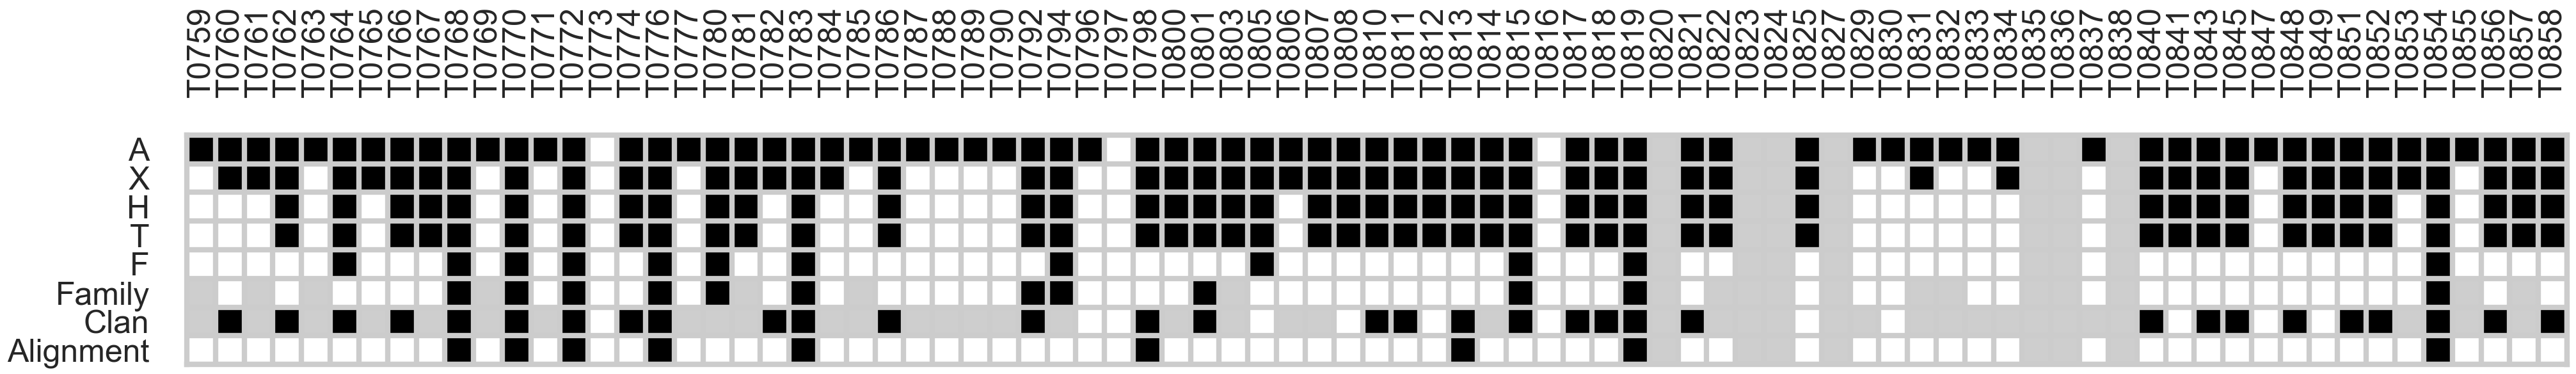
\includegraphics[width=\paperwidth]{image1.eps}
    }
%
    \caption{Overlap of the training set on each target domain of the
    test set (from T0759 to T0858). The first 5 rows of tiles
    correspond to the ECOD classification of protein domains (A-, X-,
    H-, T-, and F-groups). A black tile in any of these rows indicates
    that at least one structure from the training set belongs to the
    same ECOD group as the target. A white tile indicates that no
    structure belongs to the same group. Targets for which no ECOD
    classification is available are left empty (grey).
    A black tile in the ``Family'' row indicates that at least one
    structure from the training set belongs to the same Pfam family as
    the target. (Grey indicates that no Pfam family information is
    available for the target.) The ``Clan'' row shows similar
    information for Pfam clans. A black tile in the ``Alignment'' row
    indicates that at least one sequence in the training set aligns to
    the target sequence with an E-value smaller than $10^{-4}$. (Grey
    indicates that the protein structure is absent from the PDB database)}
    \label{Fig:summaryTable}
\end{figure*}


\subsection{Input}
The protein structure is represented by 11 density maps corresponding
to the atom types defined in Table~\ref{Tbl:atomTypes}. These atom
types are a simplification of the 20 types proposed by Huang and
Zou \citep{huang2006iterative, huang2008iterative}, to reduce the
memory footprint of the model.
The density of an atom is modeled using the function
\begin{equation}
\label{eq:rho}
\rho(r) =  \begin{cases}
               e^{-\frac{r^2}{2}}&\text{if } r\leq 2.0\text{ \AA} \\
               0                 &\text{if } r>2.0\text{ \AA} \\
            \end{cases}
\end{equation}
The atomic density is projected to the grid corresponding to its atom
type. Each grid has a resolution of 1~\AA\ and has $120\times
120\times 120$ cells.

\begin{table}[!t]
\begin{center}
\begin{tabular}{ c | l | l }
    
    Type & Description & Atoms \\
    \hline
    1 & Sulfur/selenium & CYS:SG, MET:SD, MSE:SE \\ \hline
    2 & Nitrogen (amide) & ASN:ND2, GLN:NE2, backbone N (including N-terminal) \\ \hline
    3 & Nitrogen (aromatic) & HIS:ND1/NE1, TRP:NE1 \\ \hline
    4 & Nitrogen (guanidinium) & ARG:NE/NH1/NH2 \\ \hline
    5 & Nitrogen (ammonium) & LYS:NZ \\ \hline
    6 & Oxygen (carbonyl) & ASN:OD1, GLN:OE1, backbone O (except C-terminal) \\ \hline
    7 & Oxygen (hydroxyl) & SER:OG, THR:OG1, TYR:OH \\ \hline
    8 & Oxygen (carboxyl) & ASP:OD1/OD2, GLU:OE1/OE2, \\
     & & C-terminal O, C-terminal OXT \\ \hline
    9 & Carbon (sp2) & ARG:CZ, ASN:CG, ASP:CG, GLN:CD, GLU:CD, \\
     & & backbone C \\ \hline
    10 & Carbon (aromatic) & HIS:CG/CD2/CE1, \\
     & & PHE:CG/CD1/CD2/CE1/CE2/CZ, \\ 
     & & TRP:CG/CD1/CD2/CE2/CE3/CZ2/CZ3/CH2, \\
     & & TYR:CG/CD1/CD2/CE1/CE2/CZ \\ \hline
    11 & Carbon (sp3) & ALA:CB, ARG:CB/CG/CD, ASN:CB, ASP:CB, \\
     & & CYS:CB, GLN:CB/CG, GLU:CB/CG, HIS:CB, \\
     & & ILE:CB/CG1/CG2/CD1, \\
     & & LEU:CB/CG/CD1/CD2, \\
     & & LYS:CB/CG/CD/CE, \\
     & & MET:CB/CG/CE, MSE:CB/CG/CE, \\
     & & PHE:CB, PRO:CB/CG/CD, \\
     & & SER:CB, THR:CB/CG2, \\
     & & TRP:CB, TYR:CB, VAL:CB/CG1/CG2, \\
     & & backbone CA \\ \hline    
\end{tabular}
    
    \caption {Atom types used in this work. Atoms in each group are
    identified using their standard PDB residue names and atom names.}

    \label{Tbl:atomTypes}
\end{center}
\end{table}

Figure~\ref{Fig:atomic_densities} illustrates the atomic densities for
a simple $\alpha$-helical peptide (PDB code 5eh6). This structure
contains only 6 of the 11 atom types, and only those density maps are
shown.

\begin{figure*}[!tpb]
    \centering
    \includegraphics[width=0.7\linewidth]{image2.eps}

    \caption{Representation of a protein structure (PDB code 5eh6)
    using atomic densities. The density maps are calculated according
    to Eq.~\ref{eq:rho} and rendered using Pymol \citep{PyMOL} with an
    isosurface level of $0.5$.}

    \label{Fig:atomic_densities}
\end{figure*}


\subsection{Model}
Convolutional neural networks were first proposed for image
recognition by LeCun et al.\ \citep{lecun1989backpropagation} but have
gained wider recognition after the ImageNet 2012
competition \citep{krizhevsky2012imagenet}. In this work we use 3D
convolutional networks to score protein structures. The architecture
of the model is shown in Figure~\ref{Fig:CNNModel}.  It is comprised of
three blocks of alternating convolutional, volumetric batch
normalization, and ReLU layers, followed by three fully-connected
layers with ReLU nonlinearities. The final output of the network is a
single number, interpreted as the score of the input structure.

\begin{figure*}[!tpb]
    \centering
    \includegraphics[width=\linewidth]{image3.eps}

    \caption{Schematic representation of the convolutional neural
    network architecture used in this work. Line connections across
    boxes denote the consecutive application of a 3D convolutional
    layer (``Convolution''), a batch normalization layer
    (``BatchNorm''), and a ReLU layer. Arrows between boxes denote
    maximum pooling layers (``MaxPooling''). The labels ``$\times M$''
    denote the number of filters used in the corresponding 3D
    convolutional layer. The size of all filters and maximum pooling
    domains are $3\times 3\times 3$. The grey stripes denote
    one-dimensional vectors and crossed lines between them stand for
    fully-connected layers with ReLU non-linearities. Details of the
    model parameters can be found in Supplementary Information Table~S4.}

    \label{Fig:CNNModel}
\end{figure*}

Each 3D convolutional layer takes $N$ input density maps $f$ and
transforms them using $M$ filters $F$ according to the following
formula:
$$
f^\text{out}_i (\mathbf{r}) = \sum^{N}_{j=1} \int F_i (\mathbf{r} - \mathbf{r'}) \cdot f^\text{in}_j(\mathbf{r'}) ~d\mathbf{r'}, \quad\forall i \in [1,M]
$$
In practice, these convolutions are approximated by sums on a 3D grid.
The ReLU nonlinearity is computed as following:
$$
f^\text{out}_i (\mathbf{r}) = \begin{cases}
               f^\text{in}_i(\mathbf{r}) &\text{if } f^\text{in}_i(\mathbf{r})\geq 0\\
               0                         &\text{if } f^\text{in}_i(\mathbf{r})<0\\
            \end{cases}, \quad\forall i \in [1,M]
$$
The concept of batch normalization layer was introduced by Ioffe and
Szegedy \citep{ioffe2015batch} to address the problem of internal
covariate shift (the shift in the distribution of subnetwork outputs
during training). In practice, this layer normalizes each input value
according to the mean and variance of the corresponding input within
the subset of examples used to estimate the gradient (``batch''):
$$
\hat{f}^\text{in}_k(\mathbf{r}) = \frac{f^\text{in}(\mathbf{r}) - \mu_\text{B}}{\sqrt{\sigma^{2}_\text{B} + \epsilon}}, \quad\forall k \in [1,N_\text{B}]
$$
where $\mu_\text{B}(\mathbf{r})
= \frac{1}{N_\text{B}} \sum_{k=1}^{N_\text{B}}
f^\text{in}_i(\mathbf{r})$, and $\sigma^{2}_\text{B}
= \frac{1}{N_\text{B}} \sum_{k=1}^{N_\text{B}} \left(
f^\text{in}_i(\mathbf{r}) - \mu_\text{B}
(\mathbf{r}) \right)^2$. $N_\text{B}$ is the number of examples in the
minibatch. The constant $\epsilon$ is added to avoid division by
zero. Afterwards, the output of this layer is computed by scaling the
normalized inputs:
$$
f^\text{out}_k(\mathbf{r}) = \gamma \hat{f}^\text{in}_k(\mathbf{r}) + \beta, \quad\forall k \in [1,N_B]
$$
The parameters $\gamma$ and $\beta$ are learned along with other
parameters of the network during the training.

The maximum pooling layer (``MaxPool'') is used to build a
coarse-grained representation of the input. The output of this layer
is the maximum over the cubes of size $d \times d \times d$ that cover
the input domain with the stride $l$ (distance between two consequtive
cubes along one dimension).  The output size is then approximately $l$
times smaller than the input data bounding box.  All three ``MaxPool''
layers of the model (Figure~\ref{Fig:CNNModel}) use $d=3$ and $l=2$.

During the coarse-graining procedure, the size of the individual data
grids eventually shrinks to a single cell. The flattening layer
reshapes the array of $1\times 1\times 1$ density maps to a single
vector. Afterwards, we compute several transformations using
fully-connected layers. These layers transform a vector
$\mathbf{x}_\text{in}$ as following:
$$
\mathbf{x}_\text{out} = W \cdot \mathbf{x}_\text{in} + \mathbf{b}
$$
where $W$ is a matrix and $\mathbf{b}$ is a vector, learned during the
training. Each output vector is then transformed by a ReLU layer.


\subsection{Loss functions}
The problem of decoy quality assessment is essentially a ranking
problem: we have to arrange decoys according to their similarity to
the corresponding native structure, as quantified by the GDT\_TS score
\citep{zemla2001casp4}, for instance. Such a ranking approach to the
problem of model quality assessment has recently been used by the
MQAPRank method \citep{jing2016sorting}, which, however, relies on a
support vector machine model and uses high-level features as
input.

In the present work, we define the loss function in terms of the
margin ranking loss \cite{joachims2002optimizing, gong2013deep} for each pair of decoys.
Let $\text{GDT\_TS}_i$ denote the global distance test total score of
decoy $i$ and let $y_{ij}$ be the ordering coefficient of two decoys
$i$ and $j$:
$$
y_{ij} = \begin{cases}
               1& \text{if }\text{GDT\_TS}_i \leq \text{GDT\_TS}_j \\
               -1& \text{if }\text{GDT\_TS}_i > \text{GDT\_TS}_j \\
            \end{cases}
$$
%
In this work we assume that $\text{GDT\_TS}\in [0,1]$.
Let $f_i$ denote the output of the network for decoy $i$. We use the
following expression for the pairwise ranking loss function:
$$
L_{ij} = w_{ij} \max \left[ 0, 1 - y_{ij} \cdot (f_i - f_j) \right]
$$
The term $w_{ij}$ represents the weight of each example and is defined
so that decoys with similar scores are removed from the training:
$$
w_{ij} = \begin{cases}
               1& \text{if } \left| \text{GDT\_TS}_i - \text{GDT\_TS}_j \right| > T \\
               0& \text{otherwise} \\ 
            \end{cases}
$$
where $T$ is a threshold constant set to 0.1 GDT\_TS unit.

During the training procedure we load $N_\text{B} = 9$ decoy
structures of a given target into memory (a ``batch'') and compute the
output of the network and the average loss:
$$
L = \frac{1}{N_\text{B}^2} \sum_{i=1}^{N_\text{B}}\sum_{\substack{j=1\\j\neq i}}^{N_\text{B}} L_{ij}
$$
Afterwards, we compute the gradient of the average loss with respect
to the network parameters and update them using the Adam algorithm
\citep{kingma2014adam}.


\subsection{Evaluation criteria}
We evaluate the model using various correlation coefficients of the
scores and using the loss criterion. The latter is defined, for any
given protein, as the absolute difference between the GDT\_TS of the
best decoy and the GDT\_TS of the decoy with the lowest predicted
score $f$:
$$ 
\mathrm{Loss} = \left| \mathrm{max}_i(\text{GDT\_TS}_i) - \text{GDT\_TS}_{\mathrm{argmin}_i(f_i)} \right|
$$
The correlation coefficients between the $f$ score produced by the
model and the GDT\_TS score are computed for all decoys of a given
target in the test set, and are then averaged over all targets
(per-target average). Since the value of GDT\_TS increases with the
quality of a model but the value of $f$ decreases, an ideal QA
algorithm would show a correlation coefficient of $-1$ and a loss of
$0$.


\subsection{Optimization and dataset sampling}
The parameter optimization of the model was performed using the Adam
algorithm \citep{kingma2014adam}. The gradient of the loss function
with respect to the model parameters was computed on the pairs of
models in the batch. The batch size was set to $N_\text{B} = 9$
models.

The training dataset is sampled by first choosing a random target from
the dataset, then sampling decoys of this target. One epoch
corresponds to one pass through all targets in the dataset. The decoys
are sampled in a homogeneous way, by dividing all decoys of a given
target into $N_\text{B} = 9$ bins by the value of their GDT\_TS score
and picking one decoy from each bin at random.
Precisely, decoy $i$ belongs to the bin number 
$$
1 + \left[ N_B \times \frac{\text{GDT\_TS}_i - \min(\text{GDT\_TS}) }{\max(\text{GDT\_TS}) - \min(\text{GDT\_TS})} \right]
$$
where $\max(\text{GDT\_TS})$ and $\min(\text{GDT\_TS})$ are computed on all
decoys of the chosen target.
During the training we pick $N_B$ decoys from the bins ${1 \dots N_B}$.
If a bin $k$ is empty, the decoy is picked from a non-empty bin $j \neq k$ chosen randomly.
The order of targets and the order of decoys in the bins are randomly shuffled at the end of each
epoch.


Decoy structures are randomly rotated and translated each time they
are used as input. The rotations are sampled uniformly
\citep{shoemake1992uniform} and the translation are chosen in such a
way that the translated protein fits inside the $120$~\AA${}\times
120$~\AA${}\times 120$~\AA\ input grid (see Supplementary Information for
details).

We select the final model based on its performance on a
\emph{validation subset} consisting of 35 targets (and their decoys)
picked at random from the training set and excluded from the training
procedure. The remaining 529 targets are called the \emph{training
subset}.  Figure~\ref{Fig:TrainingLoss} shows the Kendall $\tau$ and
Pearson $R$ coefficients and the loss on the validation subset over 52
epochs of training.  Models are saved every 10 epochs and we pick the
one that has the smallest loss (at epoch 40).
Table~\ref{Tbl:TrainingResults} summarizes the performance metrics on
the training and validation sets for the model at epoch 40.

\begin{figure}[!tpb]
    \centering
    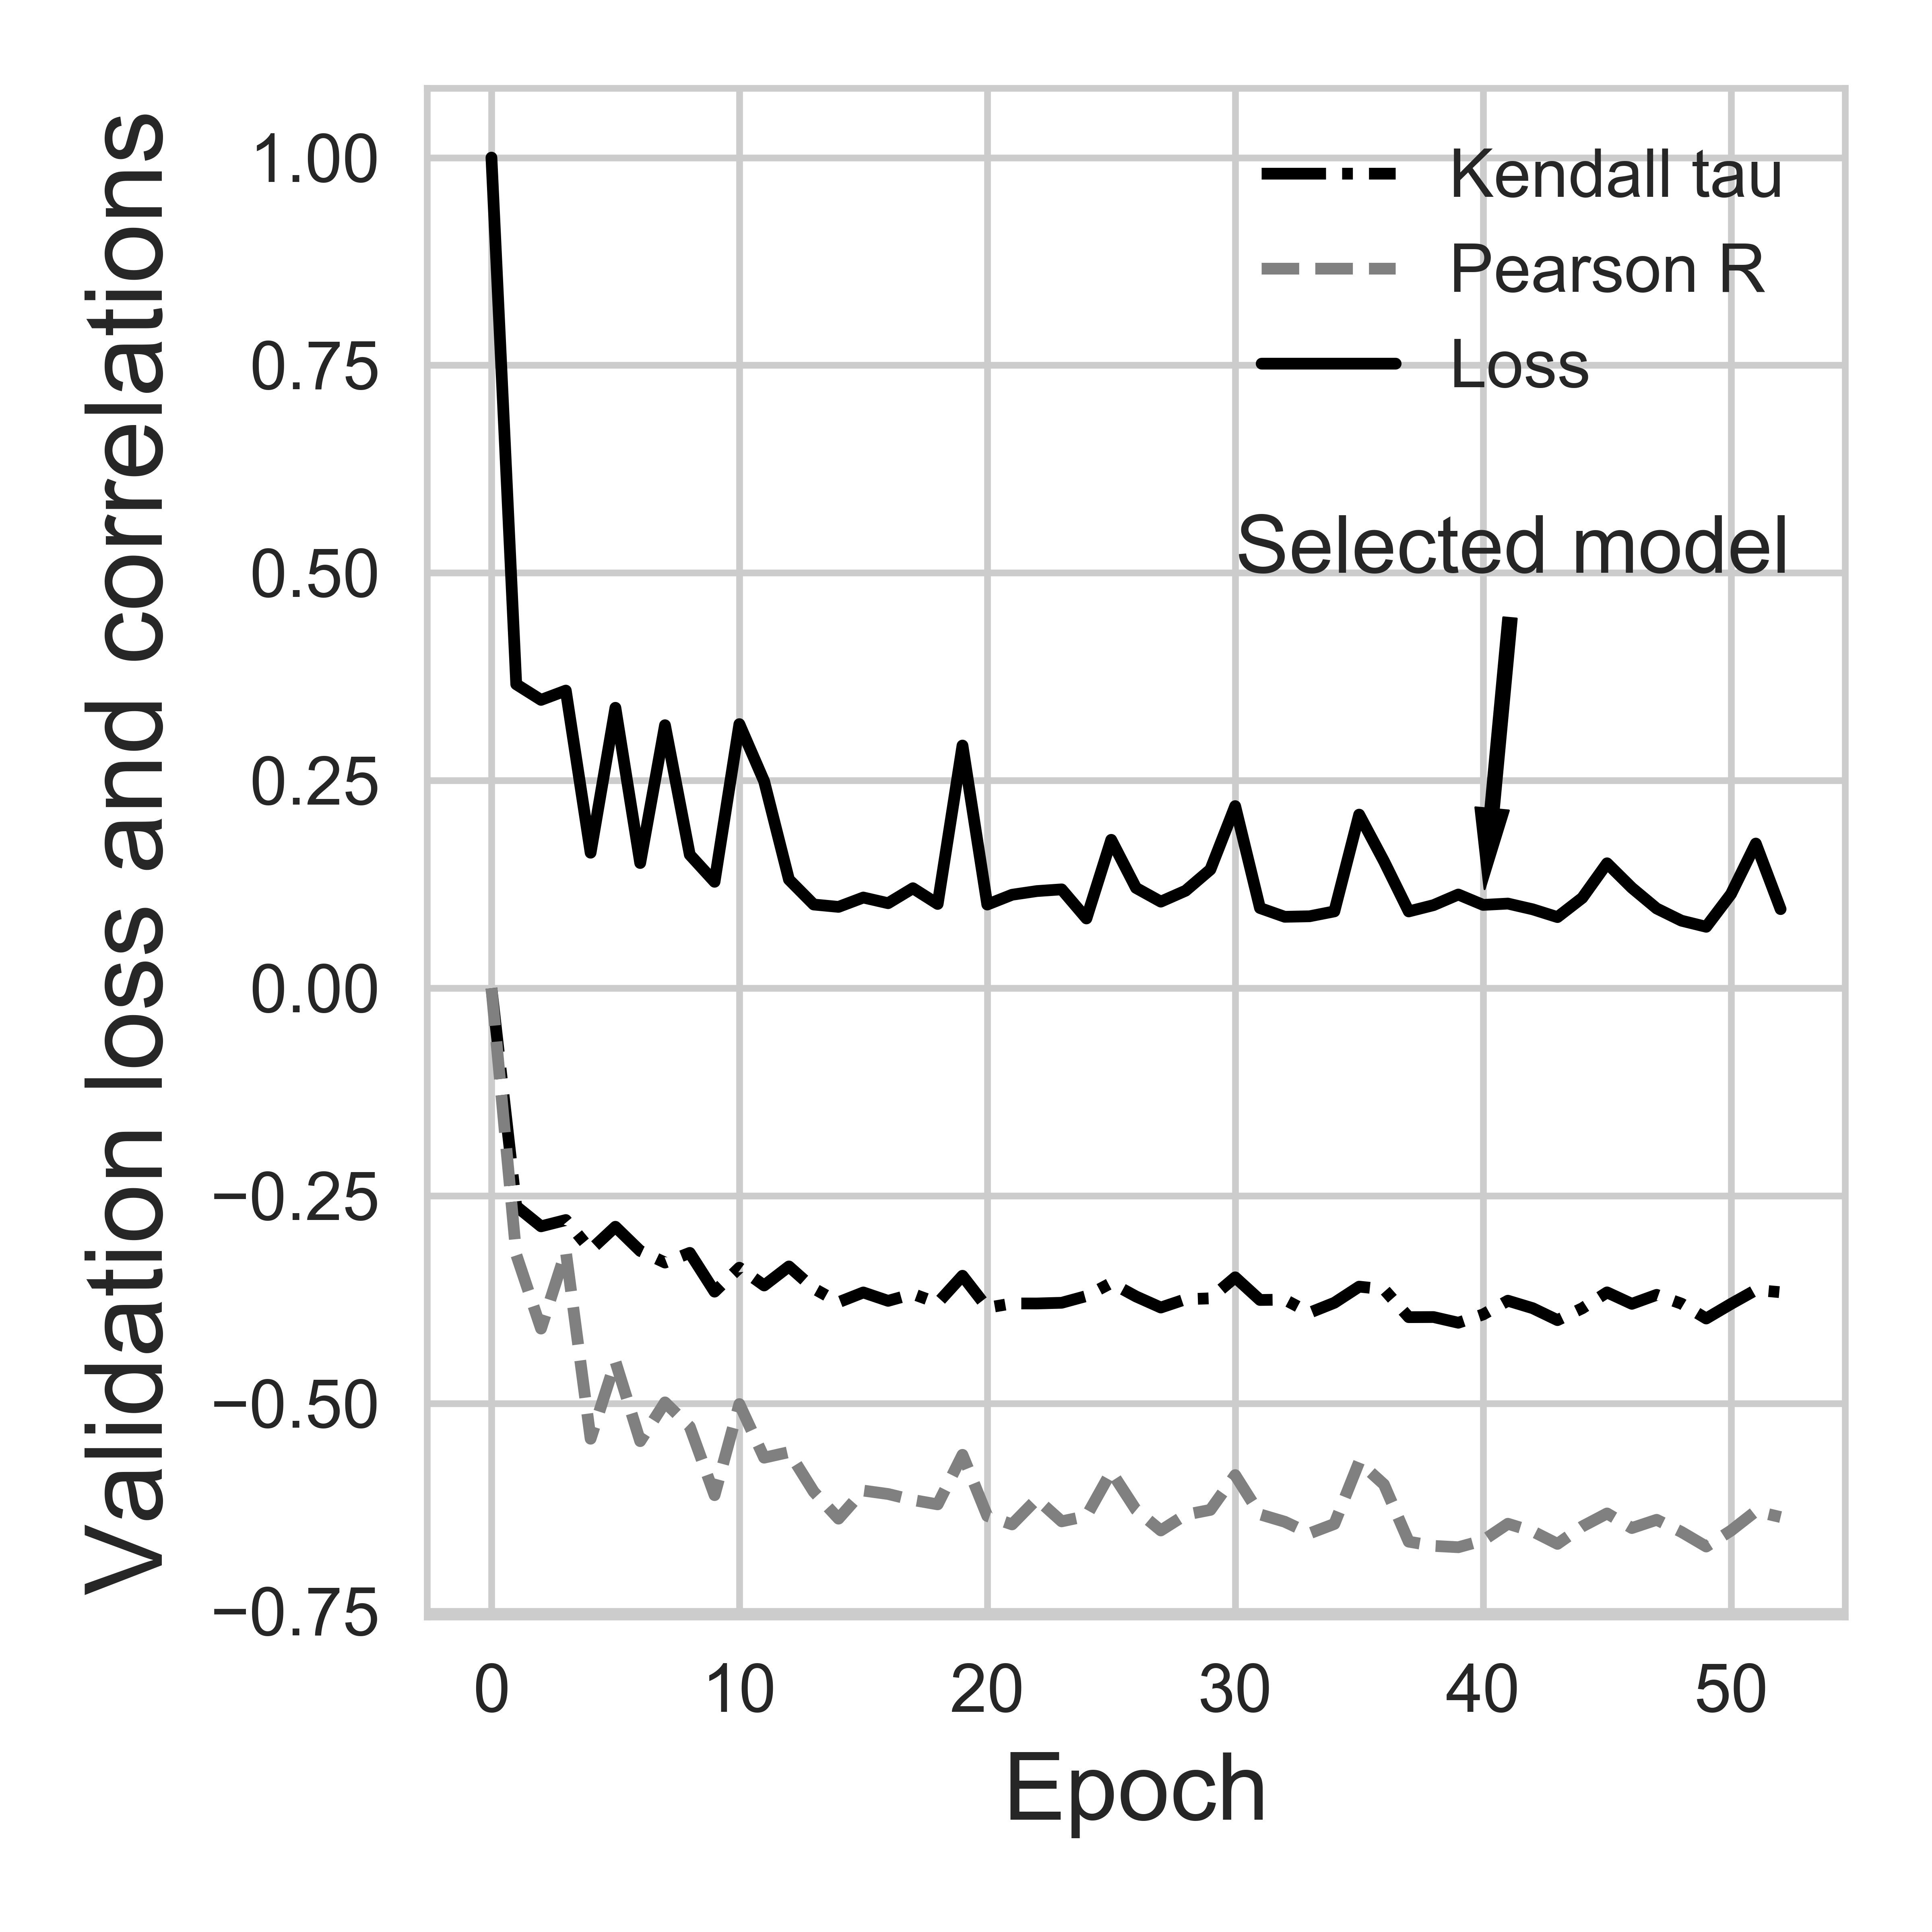
\includegraphics[width=\linewidth]{image4.eps}
    \caption{Loss, Kendall $\tau$, and Pearson $R$ coefficients
      evaluated on the validation subset during the training
      procedure.  One epoch corresponds to a cycle over all targets in
      the training subset. Models are saved every 10 epochs and the
      arrow shows the minimum validation loss for which a model was
      saved (at epoch 40).}
    \label{Fig:TrainingLoss}
\end{figure}

\begin{table}[!t]
\begin{center}
\begin{tabular}{ c | c | c | c | c }
    Data & Loss & Pearson $R$ & Spearman $\rho$ & Kendall $\tau$ \\
    \hline
    Training subset     &0.146 &0.71 &0.61 &0.45 \\
    Validation subset   &0.135 &0.71 &0.59 &0.44 \\ \hline
\end{tabular}
    \caption {Performance of the model from epoch 40 on the training
      and validation subsets.}
    \label{Tbl:TrainingResults}
\end{center}
\end{table}


\section{Results}
Ideally, the score assigned by the model to a decoy should not depend
on its position and orientation.  To allow the model to learn this
invariance, the rotational and translational degrees of freedom of all
decoy structures are randomly sampled during the training.
Figure~\ref{Fig:DecoysScoreDistribution} shows the distributions of
scores for several decoy structures of the same target (T0832),
calculated for 900 rotations and translations sampled uniformly.
While the score of a given structure is not strictly invariant under
rotation and translation, it has a relatively narrow, unimodal
distribution.  More importantly, the difference between the average
scores of two decoys is usually larger than their variances. To reduce
the influence of the choice of rotation and translation on the final
ranking, we estimate the score of each decoy from the average of 90
scores calculated for random rotations and translations. The distribution 
of the scores under rotations and translations separately is shown on 
the Fig~S4 (see Supplementary Information).

\begin{figure}[!tpb]
    \centering
    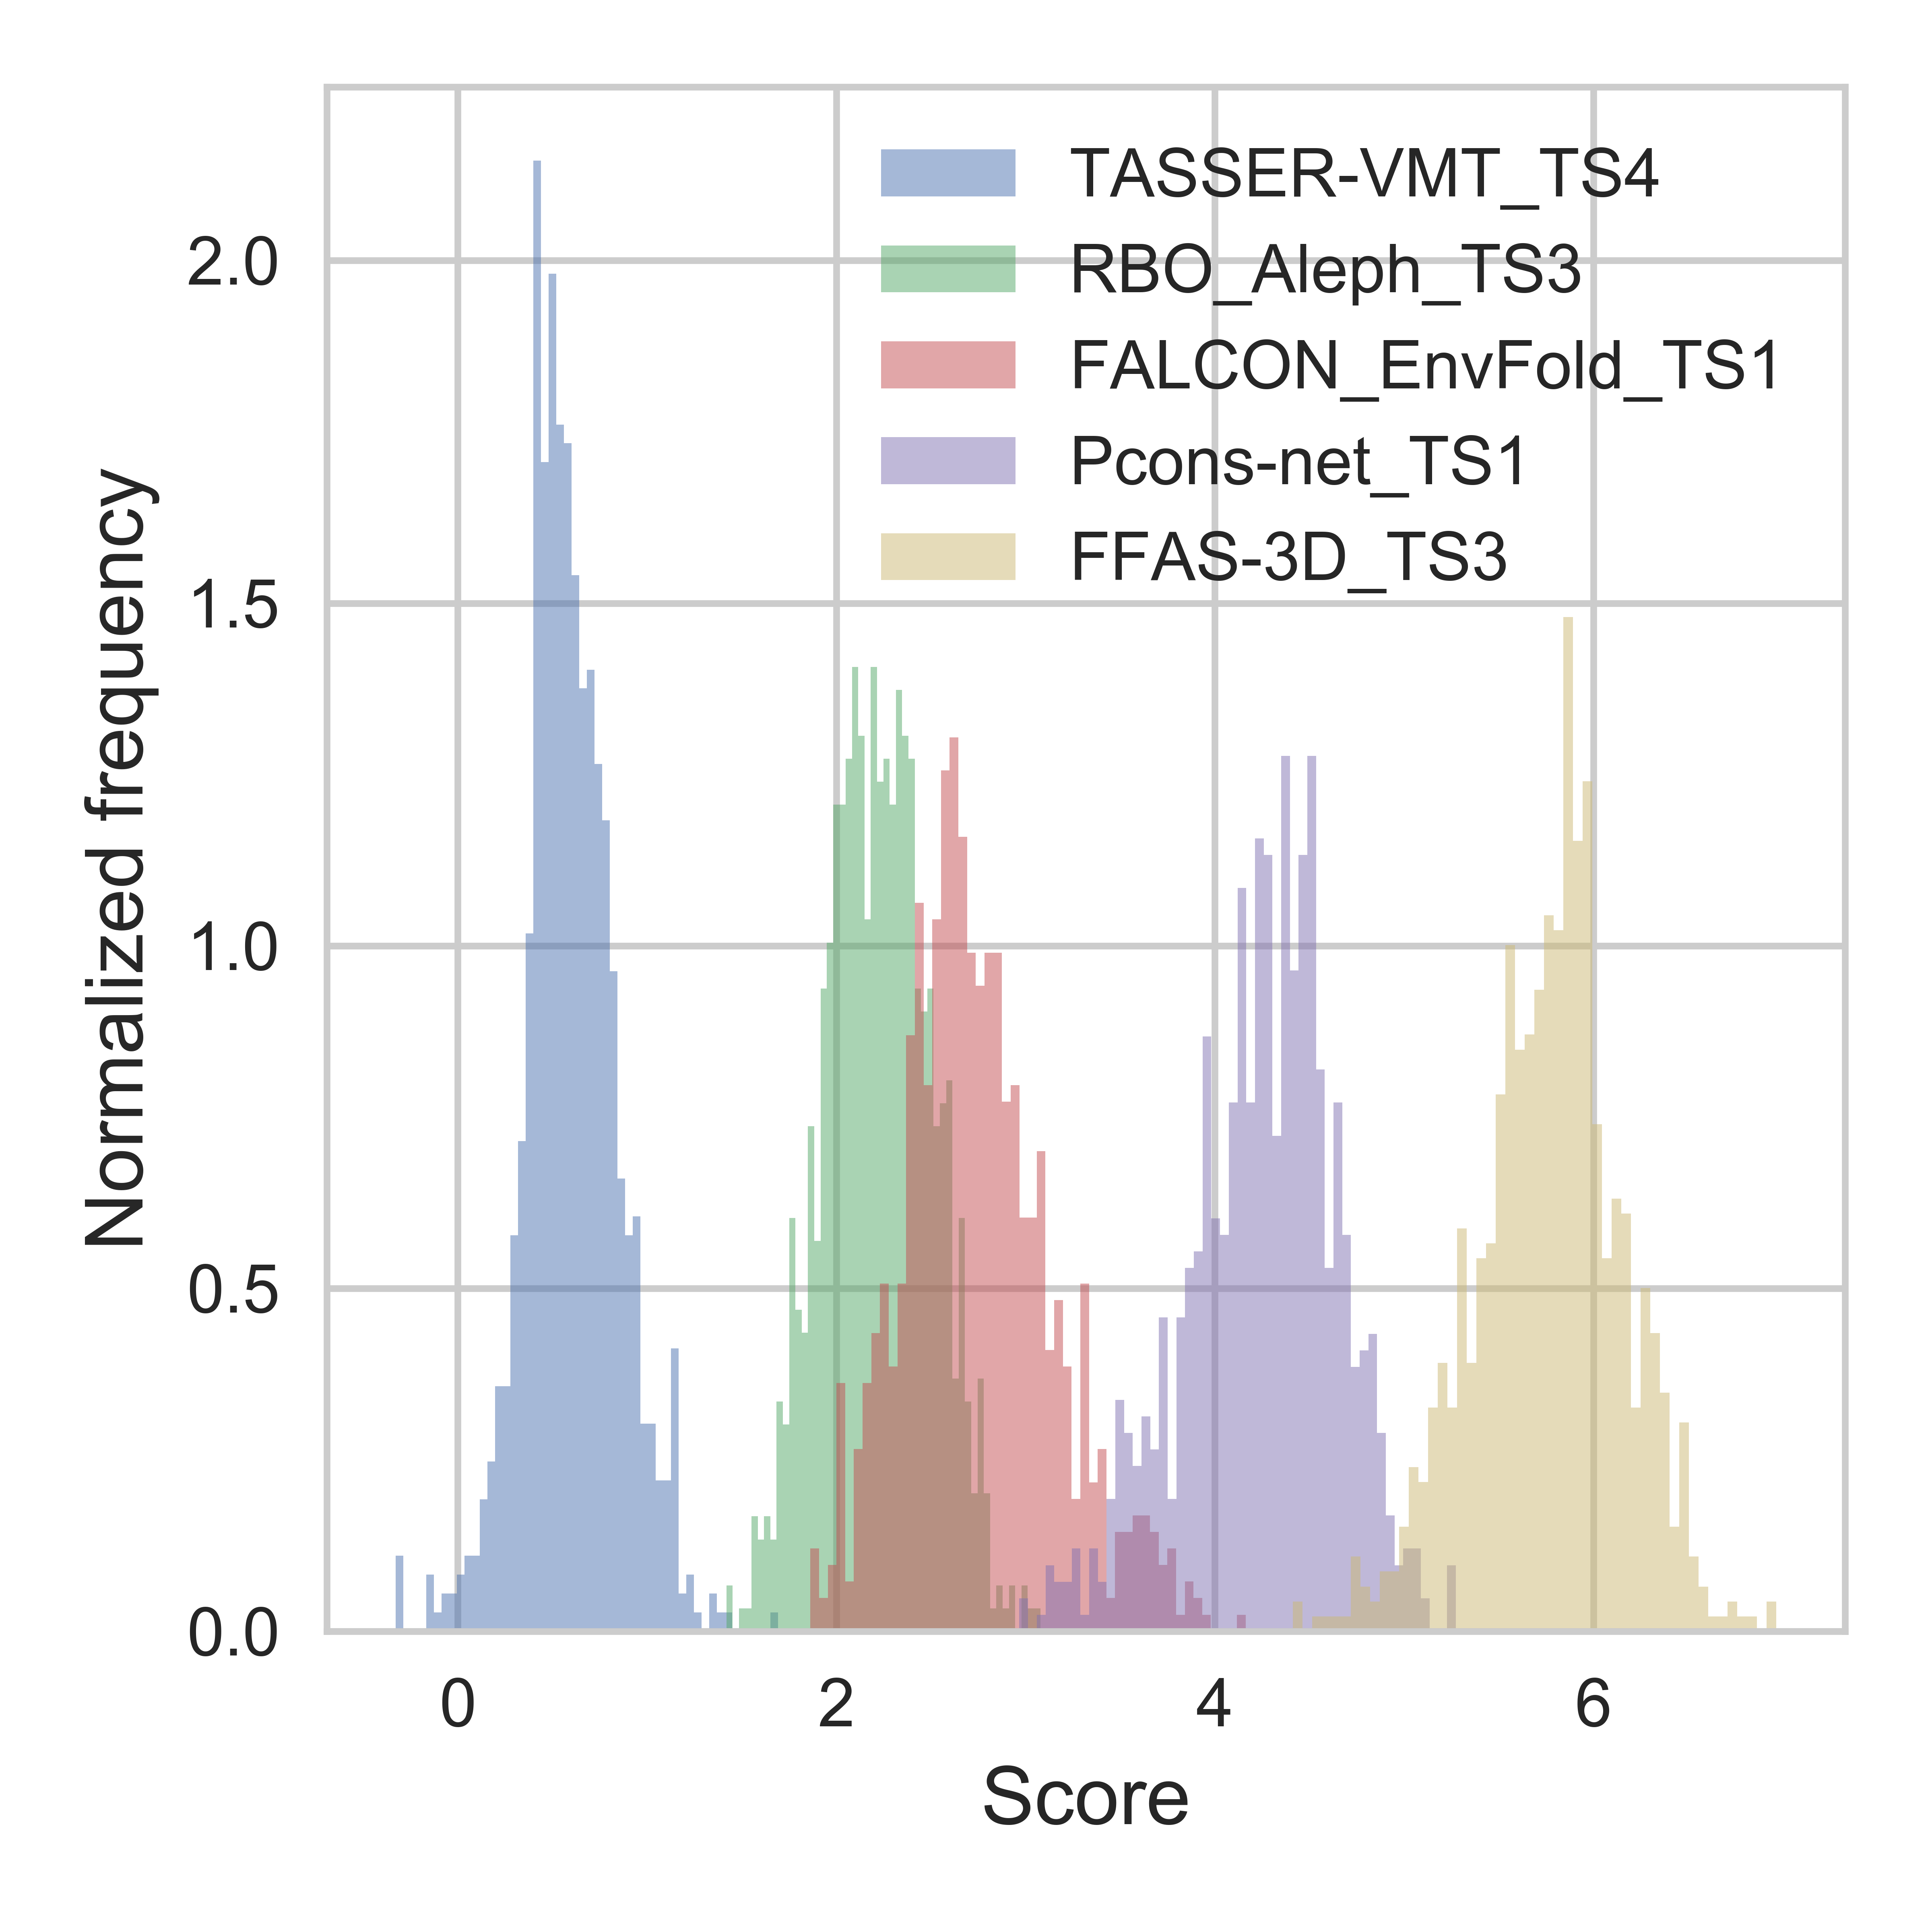
\includegraphics[width=\linewidth]{image5.eps}
    \caption{Distributions of the $f$ scores of five decoys for target
    T0832 under random translations and rotations. A lower score
    represents a higher quality.}
    \label{Fig:DecoysScoreDistribution}
\end{figure}

Table~\ref{Tbl:TestResults} shows a comparison of our model (3DCNN)
with state-of-the-art model quality assessement methods: ProQ2D,
ProQ3D~\citep{uziela2017proq3d}, VoroMQA~\citep{olechnovivc2017voromqa},
and RWplus~\citep{zhang2010novel}.
Targets T0797, T0798, T0825 are removed from this benchmark because
they were released for multimeric prediction.

ProQ2D uses carefully tuned features based on surface area
accessibilities, residue-residue contacts, predicted and observed
seconday structure, residue conservation and atomic contacts. ProQ3D
employs the same features as ProQ2D, as well as some Rosetta energy
terms~\citep{leaverfay2011rosetta}. For both ProQ2D and ProQ3D, the
features are used as input for a deep neural network to predict both
the local and global quality of the structure.
ProQ2D and ProQ3D methods are derived from ProQ2, the best-performing
single-model algorithm in CASP11, and are expected to perform better
than the original ProQ2 and ProQ3 methods.

RWplus is a representative of the widespread knowledge-based approach
to separating the native structure from its decoys, such as
DOPE~\citep{shen2006statistical}  or DFIRE~\citep{zhou2002distance}.

VoroMQA uses knowledge-based potentials that depend on the contact
surface between every pair of heavy atoms in the protein (or the
solvent).
VoroMQA uses an approach distinct from both the common
machine-learning techniques exemplified by the ``ProQ'' methods and
the knowledge-based potential techniques exemplified by the RWplus
method.

Moreover, these methods have available source codes or executables.
This allows us to re-evaluate their performance on our CASP11
benchmark, for which the decoys side chains are optimized using
SCWRL4.

\begin{table}[!t]
\begin{center}
\begin{tabular}{ c | c | c | c | c }
    MQA method & Loss & Pearson $R$ & Spearmann $\rho$ & Kendall $\tau$ \\ \hline
    \multicolumn{5}{ c }{Stage 1} \\ \hline
    ProQ3D   &0.046 &0.755 &0.673 &0.529 \\
    ProQ2D   &0.064 &0.729 &0.604 &0.468 \\
    \textbf{3DCNN} &0.064 &0.535 &0.425 &0.325 \\    
    VoroMQA  &0.087 &0.637 &0.521 &0.394 \\
    RWplus   &0.122 &0.512 &0.402 &0.303 \\ \hline
    
    \multicolumn{5}{ c }{Stage 2} \\ \hline
    VoroMQA  &0.063 &0.457 &0.449 &0.321 \\ 
    \textbf{3DCNN} &0.064 &0.421 &0.409 &0.288 \\
    ProQ3D   &0.066 &0.452 &0.433 &0.307 \\
    ProQ2D   &0.072 &0.437 &0.422 &0.299 \\
    RWplus   &0.089 &0.206 &0.248 &0.176 \\ \hline

\end{tabular}
%
    \caption{Performance comparison of our method (3DCNN) with other
    state-of-the-art model quality assessment methods on the CASP11
    dataset stages~1 and 2 (see text). The table reports the absolute,
    per-target average values of the correlation coefficients. 
    Targets T0797, T0798, T0825 were excluded from the evaluation. }
    \label{Tbl:TestResults}
\end{center}
\end{table}



\subsection{Analysis}
Deep neural networks are often thought of as ``black boxes'' that are
easy to train but difficult to intepret. Interpreting the results
obtained using these techniques may indeed be more challenging than
getting the results themselves. This difficulty of interpretation
sometimes leads to the suspiction that the neural network learns
artifacts in the data that correlate with the target results but are
not meaningful on any datasets other that those, chosen for training and evaluation.
%
In this section we attempt to show that our network learns relevant
description of a protein structure and can successfully rank decoys in the 3DRobot dataset.

First, we identify the regions of a structure that are responsible for
an increase of its score (a \emph{decrease} in its quality). If the
network has learned intepretable features of the data, we expect this
analysis to show that the regions responsible for the poor quality of
a decoy structure are those in which it deviates from the native
structure.
%
We use the Grad-CAM analysis technique proposed by Selvaraju et
al.~\citep{selvaraju2016grad}. The key idea of this technique is to
compute the gradient of the model output with respect to the output of a certain layer (``activations'' of the layer) 
and take the sum of these activations weighted by the gradient.
This highlights output regions of that layer that are both strongly
activated and highly influential on the output.
The weighted layer output is then upscaled to the same size as the input of the network. 
It indicate which parts of the input contribute the most to the gradient of the network output.
In our case we choose the ReLU layer 10, for which
the output size is $25\times 25\times 25$.
We tested the method on the outputs of the neighboring layers and
layer 10 represents the best tradeoff between interpretability and
coarseness.

\begin{figure}[!tpb]
    \centering
    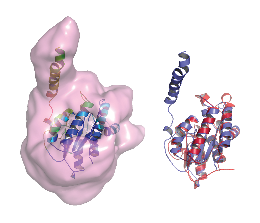
\includegraphics[width=\linewidth]{image6.eps}
    \caption{Left: The output of the Grad-CAM algorithm for the layer 10 on
    candidate structure Distill\_TS3 of target T0776. The isosurface
    shows the scaled outputs at the two-sigma level. The intensities
    of the outputs at the positions of the protein atoms are
    color-coded on the cartoon rendering of the structure, from blue
    (low intensity) to red (high intensity). Right: Cartoon
    representation of the Distill\_TS3 decoy structure (in blue)
    aligned to the native structure (in red).}
    \label{Fig:GradCAMT0776}
\end{figure}

An example of the Grad-CAM output is given in Figure~\ref{Fig:GradCAMT0776}.
In line with our scoring procedure, we perform the Grad-CAM analysis
by uniformly sampling 90 rotations and translations of the decoy. We
obtain the Grad-CAM output for each transformation and
project it onto the atoms of the decoy. 
Figure~\ref{Fig:GradCAMT0776} shows two representations of Grad-CAM result 
(for decoy Distill\_TS3 of target T0776): the
projection of the map onto the atoms of the decoy, represented as a
color-coded value on the cartoon rendering of the structure, and the
projection onto a 3D grid, represented as an isosurface. The
isosurface of Figure~\ref{Fig:GradCAMT0776} is a hollow shell containing
most of the solvent exposed region of the decoy, which indicates that
the network enforces packing: any increase in the atomic density
around the well-packed core decreases the quality of the decoy.
We also found that the weighted layer outputs are mostly zero for
structures close to the native ones (results not shown), despite the
fact that no gradient information was included in the training
procedure.

Figure~\ref{Fig:GradCAMT0776_more} shows the color-coded
values of the Grad-CAM result for the four decoys of target T0776.
We see, that the position of the N-terminal alpha-helix (which was not present in the target native structure) 
strongly influences the predictions. In case of the decoys Distill\_TS3 and 3D-Jigsaw-V5\_1\_TS2 our algorithm 
highlights this helix as the one contributing to the quality. On the other hand FALCON\_TOPO\_TS3 places this helix 
differently. This placement also better corresponds to placement of the preceeding loop in the native structure.
The Grad-CAM analysis for all the targets and selected representative decoys from CASP11 Stage2 can be found in 
Table~S4 (see Supplementary Information).
\begin{figure*}[!tpb]
    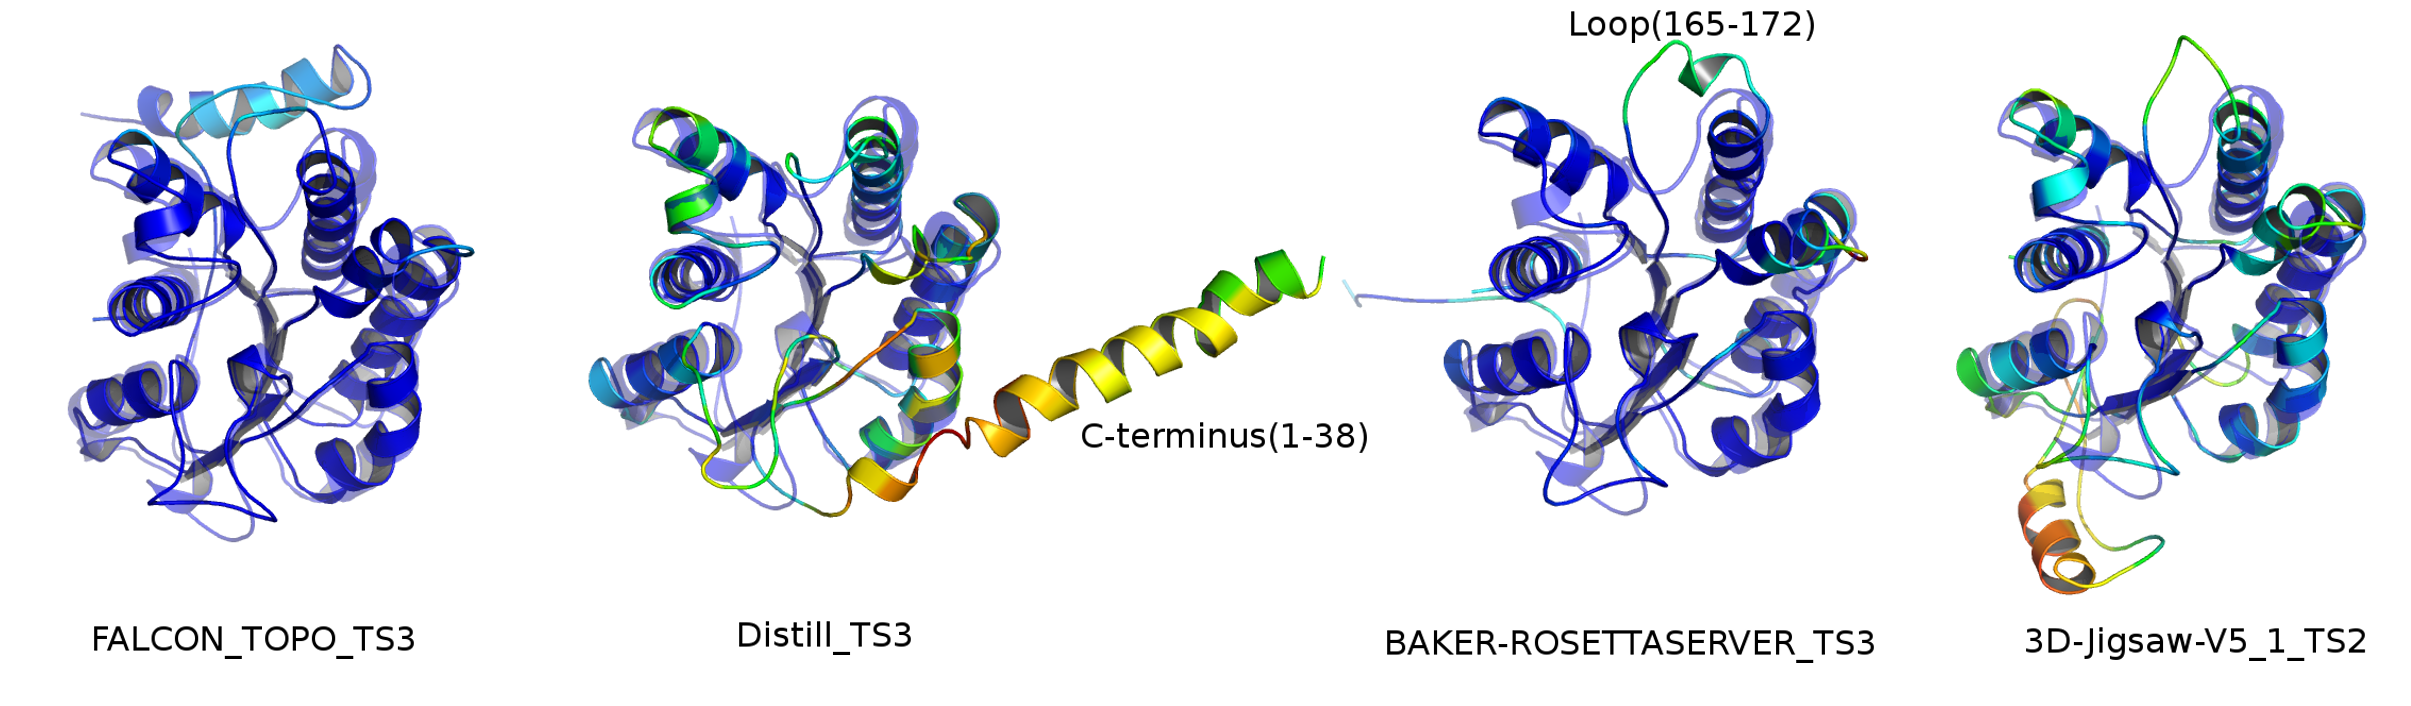
\includegraphics[width=\linewidth]{image7.eps}
    \caption{The output of the Grad-CAM algorithm for the layer 10 of the network
    projected onto the atoms of the decoys. Each decoy is aligned to
    the native structure, shown as a transparent, blue cartoon.}
    \label{Fig:GradCAMT0776_more}
\end{figure*}

To verify that the network we trained does not rely on artifacts in
the data to rank decoys, we have assessed its performance on a second,
independent dataset generated by the 3DRobot
algorithm \citep{deng20163drobot}. The decoys generated by this
algorithm are uniformly distributed within RMSD range of $[0; 12\AA]$
of the native structure and are optimized for the number of hydrogen
bonds and compactness.

The dataset consists of 300 decoys for each of the 200 non-redundant proteins. The proteins were 
selected from the PDB database with less than 20\% pair sequence identity, containing 48 $\alpha$, 
40 $\beta$ and 112 $\alpha/\beta$ signle-domain proteins with length from 80 to 250 residues. 
The absolute Pearson $R$ coefficient averaged per-target over all the
targets in this benchmark was $0.85$. Spearman $\rho$ coefficient
and Kendall $\tau$ coefficient were $0.83$ and $0.64$, respectively.
Representative examples of score versus GDT\_TS plots are shown in
Figure~\ref{Fig:3DRobotBenchmark}. We see, that the MQA method devised
in this work successfully ranks unrelated datasets.
\begin{figure}[!tpb]
    \centering
    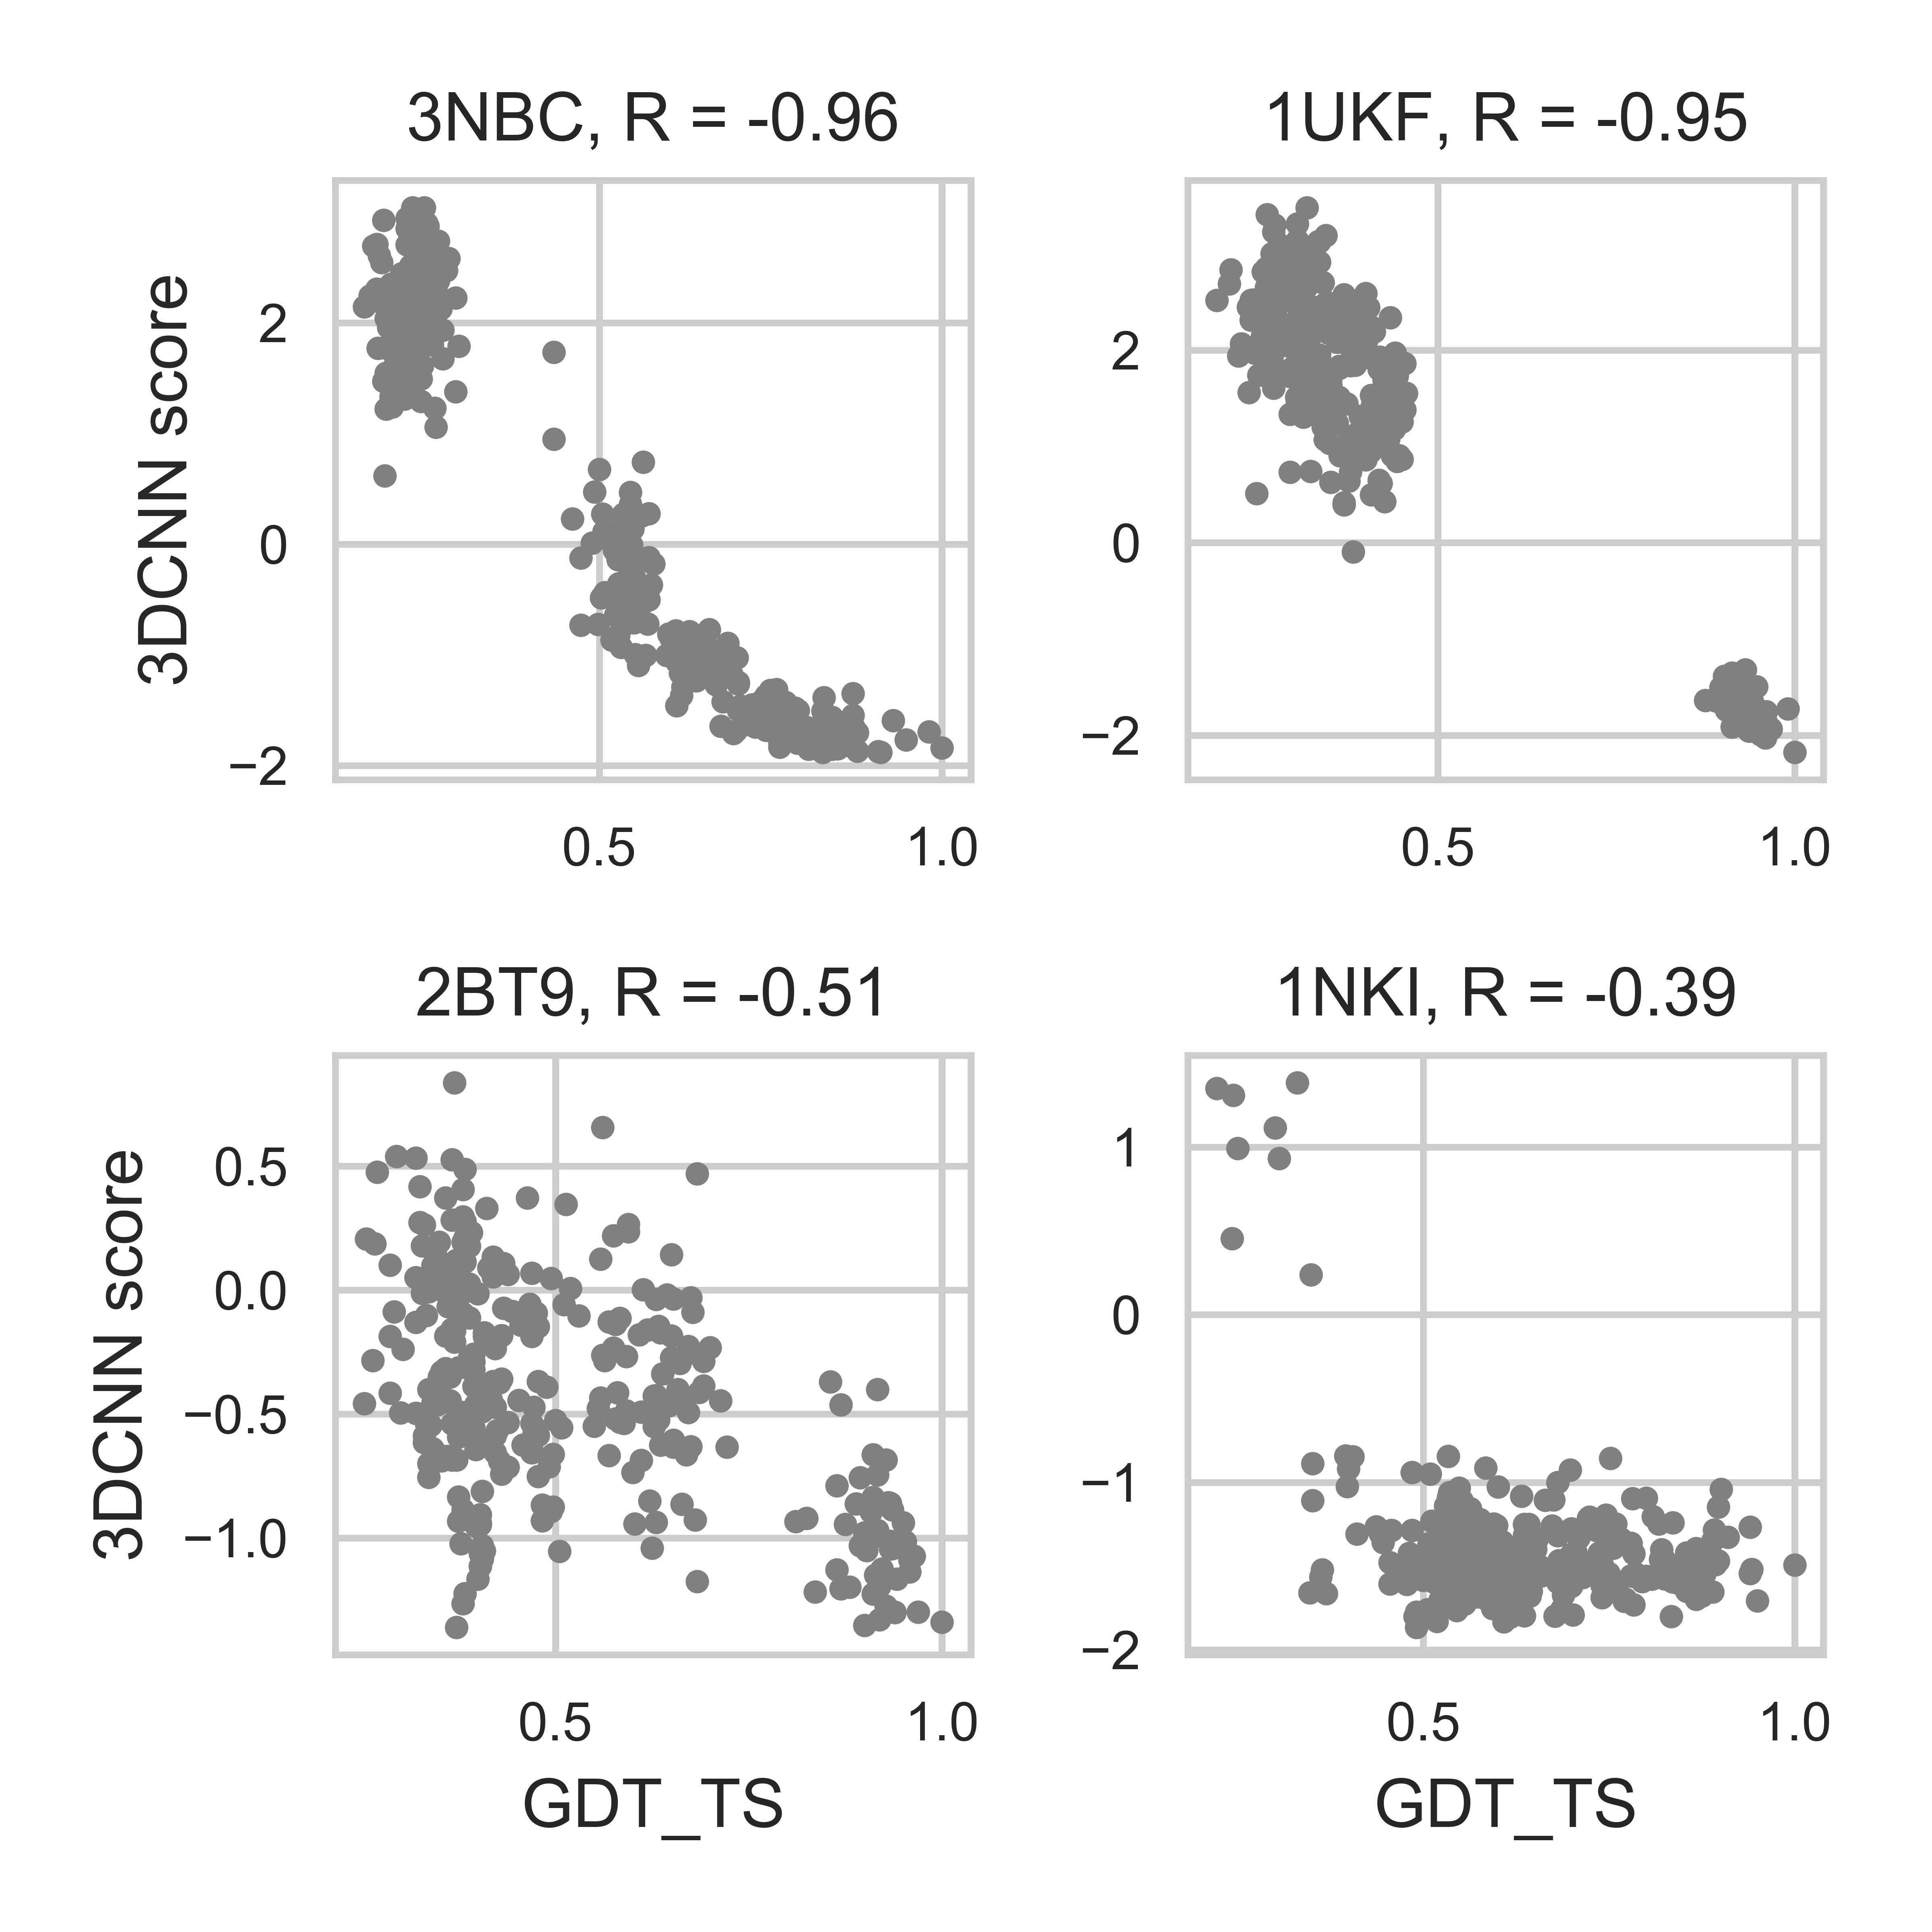
\includegraphics[width=\linewidth]{image8.eps}
    \caption{The plots of score versus GDT\_TS for two best correlated targets and two
    least correlated targets in the 3DRobot benchmark.}
    \label{Fig:3DRobotBenchmark}
\end{figure}


\section{Discussion}

In this work we showed that it is possible to construct an algorithm that learns to assess the quality of protein models from 
raw representation of the model. Our work used the atom types densities as such representation, however it is clear that 
any other physical quantity defined on the grid can be employed. The examples of such quantites are electrodymanic potential and 
water oxygen density distribution. So far, no other quality assessment method was able to include these 
crucial properties of the solute.

This work also identified some important issues: only approximate score invariance under transformations and the difficulty of 
interpretation of the results. The invariance problem can be solved using the recently published approach by Worral et al. \citep{worrall2016harmonic}.
They restricted the space of coefficient of the convolutional filters to the circular harmonics to attain eqivariance of transformations at each layer 
of the network under rotations. The layerwise equivariance then leads to the invariance of the final output.

The interpretation difficulty of deep neural networks is still an important research problem in machine learning. However, the recently 
published approach to quantify interpretability \citep{bau2017network} of deep learning models indicates the rapid advancements in this field. 
The authors of this approach used the exhaustively labeled image dataset, that contains the bounding boxes and labels for 
fine-grained features, such as body parts or car parts. In the case of protein models such labels are readily available: 
the secondary structure elements, amino-acids, hydrogen bonding network and disulfide bonds, as well as others.

Alltogether, we believe that this work opens the way to directly use the information about protein environment, aleviates the need to 
engineer features and shows that the drawbacks of this approach can be solved with the further research. 

\section{Acknowledgements}
\section{Funding information}

\bibliography{citations.bib}
\bibliographystyle{natbib}


\end{document}
